\section{Introduction}\label{introduction}

This program is an adaptation of the \gls{post}. It is a program to optimize a 3
\glspl{dof} trajectory of a vehicle, e.g.~a rocket ascending through the
atmosphere.

\gls{post} was written in 1970 by the Martin Marietta Corporation for \gls{nasa}. The program is written in Fortran 4 and was mainly developed to
simulate the space shuttle, it was later built upon and greatly improved\cite{PostHistory}. Its successor, POST2, is still in use today, for example
for the Artemis program or for Perseverance\cite{PostApp}.

This project tries to use the original user manuals, which are now publicly
available (see \cref{further-reading}) to rewrite the program in a more modern programming
language: Rust. While I tried to stay close to the original, there are a few
differences. Also, only the most important features of the program were
incorporated for now, but more features can be added in the future. This is
discussed further in \cref{differences-to-the-original}.

Special thanks goes to Prof.~Dr.~Marco~Schmidt, which gave me the opportunity
to work on this project as a university course.

The manual is structured as follows: In \cref{overview}, an overview of the implementation is given. How to use the
project is described in \cref{usage}. The differences to the original and the programming language used
is discussed in \cref{discussion}. Lastly, notes about the ongoing development are given in \cref{development}.

\section{Overview}\label{overview}

This section will give an overview of the program. The program is split into
two parts. The simulation and the optimization. The optimization is tweaking
the parameters of the simulation and executes it repeatedly to search for the
optimal trajectory. This macro logic is shown in \cref{macrologic}.

\begin{figure}[!ht]
  \centering
  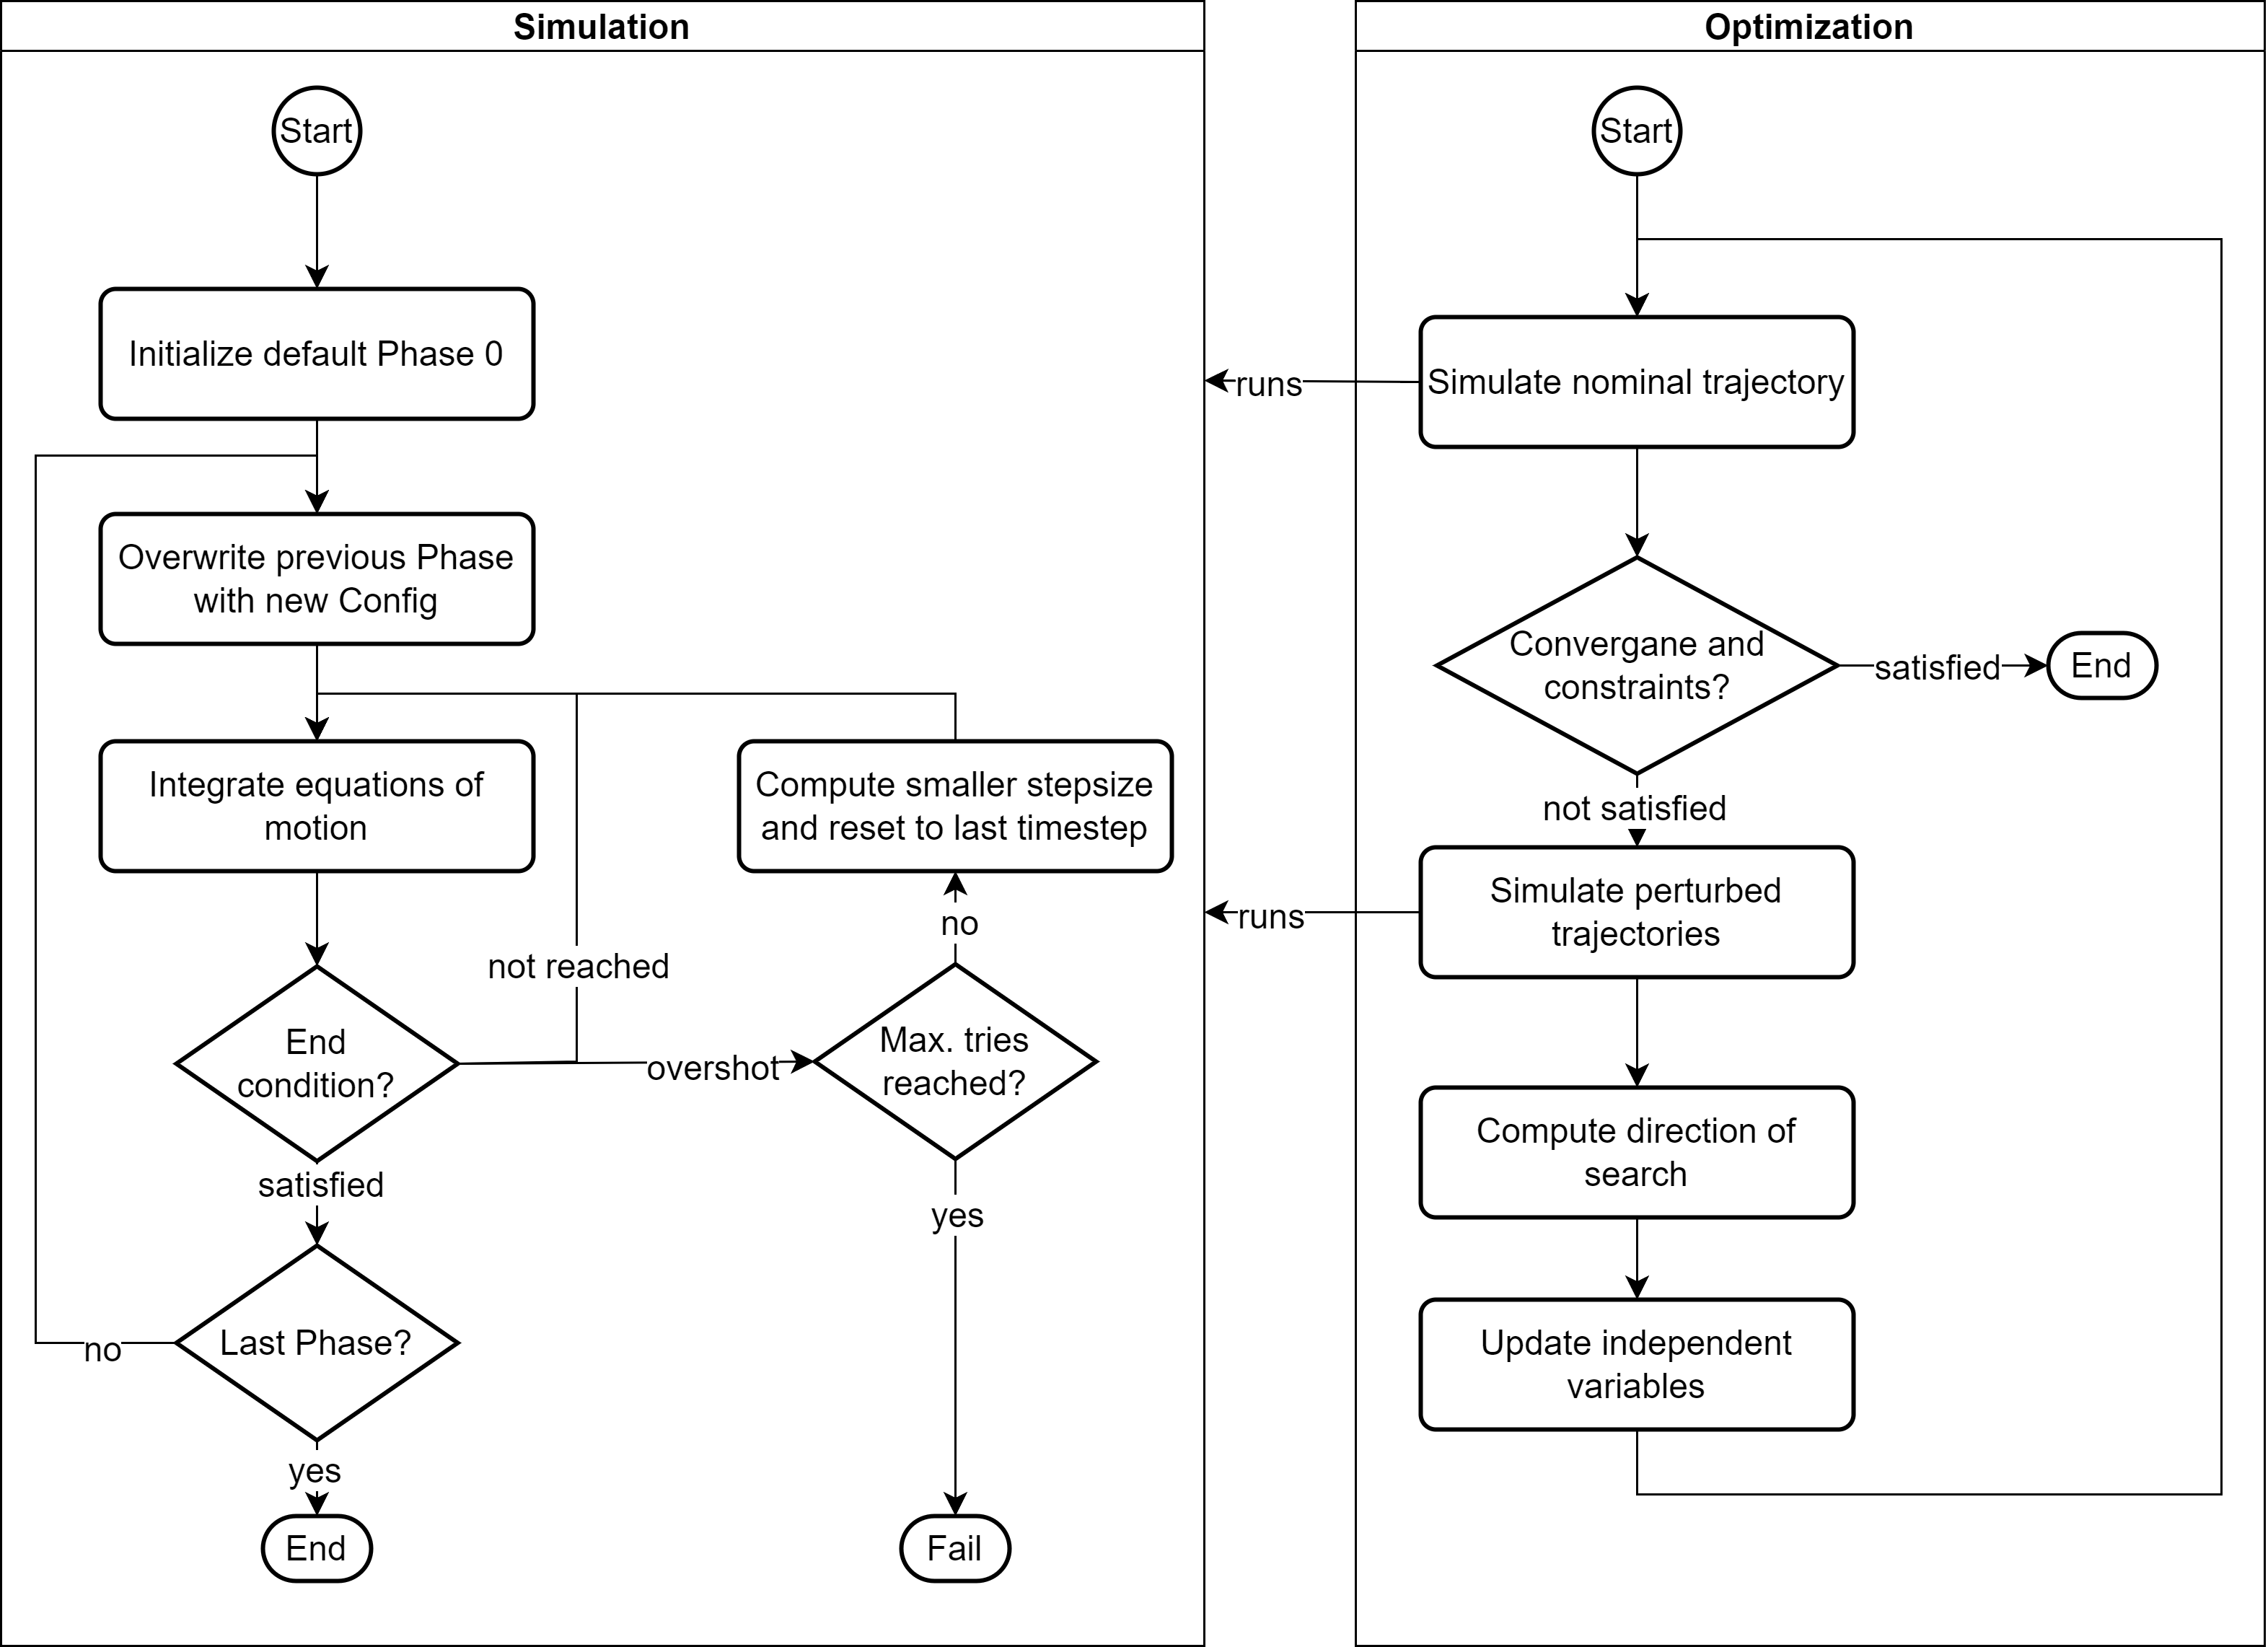
\includegraphics[width=\textwidth]{images/macrologic.png}
  \caption{Program macrologic.}
  \label{macrologic}
\end{figure}

First, I will show how the simulation works in general, then I will give a few
more details on the equations of motion. Next, I will give an idea on how the
optimization works. Lastly, I give an overview of the original documentation,
where each part is explained in great detail.

\subsection{Simulation}\label{simulation}

The simulation consists of multiple phases, each split by an event. One
example is shown in \cref{example}. This actually the example which was used to validate the
implementation of this project.

Each phase consists of two sets of variables: the configuration parameters and
the simulation variables. The configuration parameters define the vehicle and
its environment, while the simulation variables are calculated by the
simulation for each time step. To understand the concept better, here are some
examples for configuration parameters:
\begin{itemize}
  \item Planet model
  \item Wind strength / direction
  \item Launch latitude
  \item Vehicle structure mass
  \item Vehicle pitch rate
  \item Simulation step size
  \item etc.
\end{itemize} And here are some examples for simulation variables:
\begin{itemize}
  \item Simulation Time
  \item Position
  \item Acceleration
  \item Mass
  \item Euler Angles
  \item Aerodynamic Forces
  \item etc.
\end{itemize}

These are described in detail in \cref{usage}.

\begin{figure}[!ht]
  \centering
  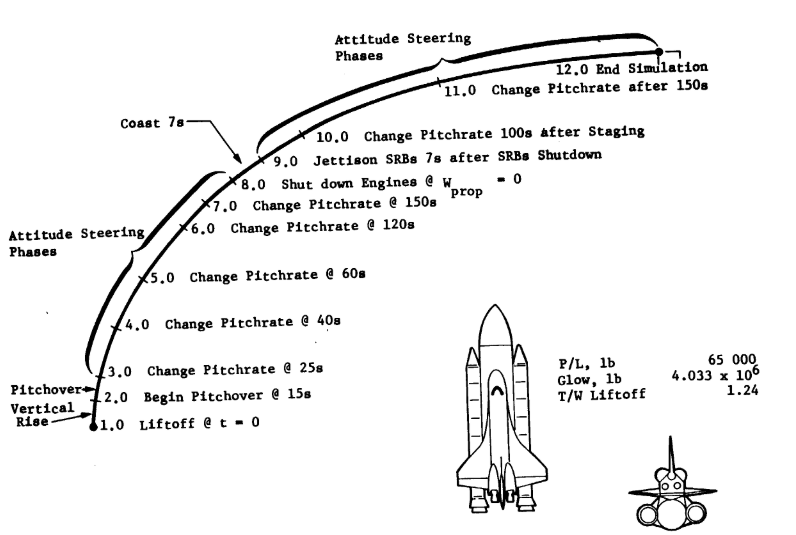
\includegraphics[width=\textwidth]{images/example.png}
  \caption{Example simulation split into phases by events from \cite[Fig. 28]{PostSummary}.}
  \label{example}
\end{figure}

Each event is always some simulation variable reaching a specified value, both
of which can be defined by the user in the configuration. At the beginning of
each phase, the user can define changes in the configuration.

The simulation executes each phase in the following way:

First, the phase is initialized with the configuration and end state of the
previous phase, then it is updated with its own configuration parameters.

Next, an integrator is integrating the equations of motion and the mass flow
for a fixed time step. The next chapter will detail the equations of motion.
In the equations of motion, the simulation state, consisting of all simulation
variables, is slowly build step by step.

After each time step, the simulation checks the termination condition for the
current phase. If the specified value is reached (within a margin), the phase
is terminated. If the simulation overshot the termination condition, it will
compute a smaller time step and redo the simulation step.

\subsubsection{Coordinate Frames}\label{coordinate-frames}

There are 4 coordinate frames used. These are the inertial frame,
earth-relative frame, launch frame and body frame.

\begin{description}
  \item[Inertial Frame] The inertial frame is located at earth's center and is
    fixed in inertial frame. \(z_I\) points towards the North Pole and the \(x_I\), \(z_I\)
    plane intersects Greenwich at time zero.
  \item[Earth-relative Frame] The earth-relative frame is the same as the
    inertial frame at time zero, but rotates together with the earth. This means
    the difference of two velocity vectors in both frames is earth's velocity at
    that point.
  \item[Launch frame] The launch frame is initialized at the launch location and
    planar to the oblate earth's surface with \(z_L\) pointing towards the North Pole,
    except it is rotated by the \json{"azimuth"} parameter specified by the user. The frame is shown in \cref{launch-frame}. The launch frame is an inertial frame, meaning it does not
    rotate with earth. It is used as a fixed reference point for the Euler angles.
  \item[Body frame] The body frame is located at the vehicles center of mass. \(x_B\)
    points in the direction of flight, rotation around this axis corresponds to roll.
    Rotations around \(y_B\) corresponds to pitch and rotations around \(z_B\) corresponds
    to yaw. The frame is defined arbitrarily, only the user needs to be consistent with its
    usage, as the user defines the thrust direction and aerodynamic coefficients.

    \textbf{Attention:} The orientation using the euler angles are in the order
    roll-yaw-pitch. Read more about the coordinate systems and transformations in \cite[Sec. III]{PostFormulation}.
\end{description}

\begin{figure}[!ht]
  \centering
  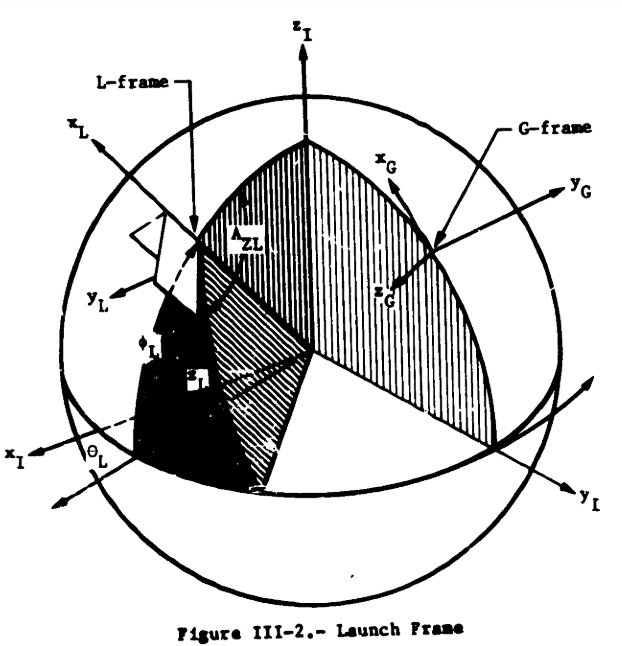
\includegraphics[width=0.5\textwidth]{images/launch-frame.png}
  \caption{The Inertial Launch Frame (G-Frame not used) from \cite[Fig. III-2]{PostFormulation}.}
  \label{launch-frame}
\end{figure}

\begin{figure}[!ht]
  \centering
  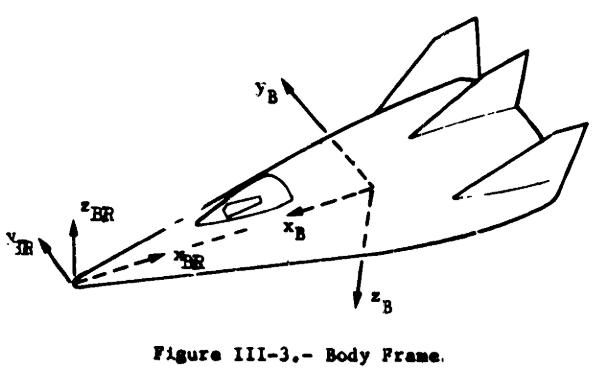
\includegraphics[width=0.5\textwidth]{images/body-frame.png}
  \caption{The Body Frame (BR-Frame not used) from \cite[Fig. III-3]{PostFormulation}.}
  \label{body-frame}
\end{figure}

The original program also includes some other coordinate frames which are not
used by this implementation.

\subsubsection{Equation of Motion}\label{equation-of-motion}

The equations of motion are the heart of the simulation. They are simple
differential equations describing the motion of the vehicle. As the program
only uses 3 \glspl{dof}, they only describe the translational movement:
\[
  \begin{array}{ll}
    \dot r_I & = v_I                              \\
    \dot v_I & = [IB]^{-1}(A_{TB} + A_{AB}) + G_I
  \end{array}
\]

The calculation of each part is outlined in the following paragraphs to give a
rough understanding of the simulation, but many details are omitted. More
details can be found in \cite[Sec. VI-4]{PostFormulation}.

\paragraph{Orientation}

The transformation from the inertial to the body frame \gls{IB} depends on the inertial Euler angles and the launch coordinate frame
(L-Frame). The Euler angles are defined with respect to the launch frame.

The Euler angles are each computed by three cubic polynomials \[
  \alpha = c_0 + c_1y + c_0y^2 + c_1y^3.
\] The coefficients \(c_i\) can be defined by the user. The variable
\(y\) is some simulation variable, which can be also picked by the user.
Each angle \(\alpha\) (roll, yaw \& pitch) has a separate polynomial and can be
configured separately.

\paragraph{Acceleration due to Thrust}

The thrust of each engine \gls{T_i} is calculated with \[
  T_i = T_{vac, i} - A_{E,i} \cdot p(h),
\] where \gls{T_vac} and \gls{A_E} are specified by the user, and \gls{p} is calculated with the atmospheric model. The acceleration due to
thrust in the body frame
\gls{A_TB} is then calculated with \[
  A_{TB} = \frac1m\sum_{i}^{N_{eng}} T_i
  \begin{bmatrix}{}
    \cos i_p \cos i_p \\
    \sin i_y          \\
    \cos i_y \sin i_p
  \end{bmatrix}_i,
\] \gls{i_p} and \gls{i_y} are specified by the user for each engine, which define the angles
between the thrust vector and the body frame.

Additionally, the mass flow is calculated with \[
  \dot m = \sum_{i}^{N_{eng}} T_{vac, i}\cdot I_{sp, i}\cdot g_0 .
\]

\paragraph{Acceleration due to Aerodynamic Forces}

The acceleration due to aerodynamic forces in the body frame \gls{A_TB} is calculated with \[
  A_{AB} = \frac1mq(h)S
  \begin{bmatrix}{} -C_A \\
    C_Y     \\
    -C_N
  \end{bmatrix},
\] where \gls{q} is calculated with the atmospheric model. \gls{S} is specified by the user.

\gls{C_A} and \gls{C_N} are calculated with \[
  A_{AB} = \frac1mq(h)S
  \begin{bmatrix}{} C_A \\
    C_N
  \end{bmatrix} = \begin{bmatrix}{}
    \cos\alpha & -\sin\alpha \\
    \sin\alpha & \cos\alpha
  \end{bmatrix}\begin{bmatrix}{} C_D \\
    C_L
  \end{bmatrix},
\] where \gls{C_D}, \gls{C_L} and \gls{C_Y} are specified by the user using tables.

The tables can be 1D, 2D or 3D, which are then interpolated using a simulation
variable, which is also specified by the user.

\paragraph{Acceleration due to Gravity}

The acceleration due to gravity is calculated with the gravity model. There
are three different gravity models available:
\begin{itemize}
  \item Spherical Model
  \item 1960 Fisher Model
  \item Smithsonian Model
\end{itemize}

Each model calculates using simple gravitational harmonics \(J_i\),
where \(J_1 = \mu\), the earth's gravitational constant. The spherical
model uses a spherical earth model and therefore only the gravitational
constant \(mu\). The 1969 Fisher model uses an oblate spheroid and
harmonics up to \(J_2\), while the Smithsonian Model includes harmonics
up to \(J_4\).

\paragraph{Atmospheric Model}

The atmospheric model used is the 1962 U.S. standard atmosphere model with a
few changes for above 90 km.

\subsection{Optimization}\label{optimization}

The optimization algorithm is detailed in the formulation manual. A rough
sketch of the algorithm is as follows:

\begin{enumerate}
  \def\labelenumi{\arabic{enumi}.}
  \item First, the nominal trajectories are simulated.
  \item Now, convergence is tested. If the problem converged, we found the
        optimal solution.
  \item If not, we simulate a slightly perturbed trajectory for each independent
        variable.
  \item With these small perturbations, the dependency of the cost function (our
        optimization goal) regarding the independent variables can be calculated. This
        is called the cost gradient.
  \item The same can be done for the constraints. This is called the sensitivity
        matrix.
  \item Next we use the cost gradient to calculate the optimization step size and
        direction, which is how the independent variables should be changed to
        optimize our problem.
  \item We use the calculated step size and direction to update our independent
        variables.
  \item Next we calculate the constraint step size and direction, which is how
        the independent variables should be changed to honor the constraints.
  \item We use the calculated step size and direction to update our independent
        variables again.
  \item Then, we repeat the process.
\end{enumerate}

\subsection{Further reading}\label{further-reading}

The program is based on the manual published in April 1975. It includes three
volumes:
\begin{enumerate}
  \item Volume 1: Formulation manual\cite{PostFormulation}
  \item Volume 2: Utilization manual\cite{PostUtilization}
  \item Volume 3: Programmer's manual\cite{PostProgrammers}
\end{enumerate}

Volume 1 is the most important one explaining the working principle and
formulas used. Volume 2 explains the usage of the original program, which
includes a few bits of extra information and an example which was important
for this project. Volume 3 explains the program's structure and was only used
a little to get an overview.

For further explanations of this project, look into these manuals. For
convenience, I included the manuals \href{https://github.com/TiborVoelcker/post/tree/master/docs/original-manuals/}{here}.

There also exists a Program summary document\cite{PostSummary} published in 1977.

Additionally, there exists a bit of documentation about the various additions,
like
\begin{itemize}
  \item 6 \glspl{dof} capabilities\cite{Post6DFormulations}
  \item Parallelization\cite{Post3D}
  \item and interplanetary missions (Volume 1\cite{IPOSTUsers}, Volume 2\cite{IPOSTAnalytic}, Volume 3\cite{IPOSTProgrammers} and Volume 4\cite{IPOSTSample}).
\end{itemize}

These were not used for this project.

\section{Usage}\label{usage}

The tool's usage is very basic. It consists of one executable, which needs to
be called with the file path to a configuration file, which is detailed below.

Until a build pipeline is implemented, the tool needs to be build first. For
this, the rust compiler and the cargo tool needs to be installed\footnote{\url{https://www.rust-lang.org/tools/install}}.

To build the tool, run
\begin{lstlisting}[language=sh]
 $ cargo build --release
\end{lstlisting}
in the project's directory. Then you can execute the script. Type
\begin{lstlisting}[language=sh]
 $ target\release\post.exe --help
\end{lstlisting}
to find out about the options of the \gls{cli}.

You can run the simulation with:
\begin{lstlisting}[language=sh]
 $ target\release\post.exe --config <config filepath>
\end{lstlisting}

This will write the time, position, velocity, altitude, and propellant mass
for each time step to the standard output, as seen below:
\begin{verbmd}
  \begin{verbatim}
Starting Phase 1
Time: 1
Position:
  ┌          ┐
  │   915482 │
  │ -5529976 │
  │  3043398 │
  └          ┘


Velocity:
  ┌     ┐
  │ 404 │
  │  65 │
  │   1 │
  └     ┘


Altitude: 1
Prop mass: 1014475

Time: 2
Position:
  ...
 \end{verbatim}
\end{verbmd}

Alternatively, the tool can be build and executed in one command with the \lstinline{cargo run} command.

\paragraph{Plotting tool}

To plot the simulated trajectory, you can pipe the output to the included
plotting tool. For this, Python needs to be installed. The tool was
implemented with Python 3.12. Then, install the requirements with
\begin{lstlisting}[language=sh]
 $ pip install -r sim\src\utils\plot\requirements.txt
\end{lstlisting}

Then, the simulated trajectory can be piped to the plotting tool with:
\begin{lstlisting}[language=sh]
 $ target\release\post.exe --config <config filepath> | python sim\src\utils\plot\plot.py
\end{lstlisting}

You should see a window open to show the simulated trajectory like in \cref{example-plot}.

\begin{figure}[!ht]
  \centering
  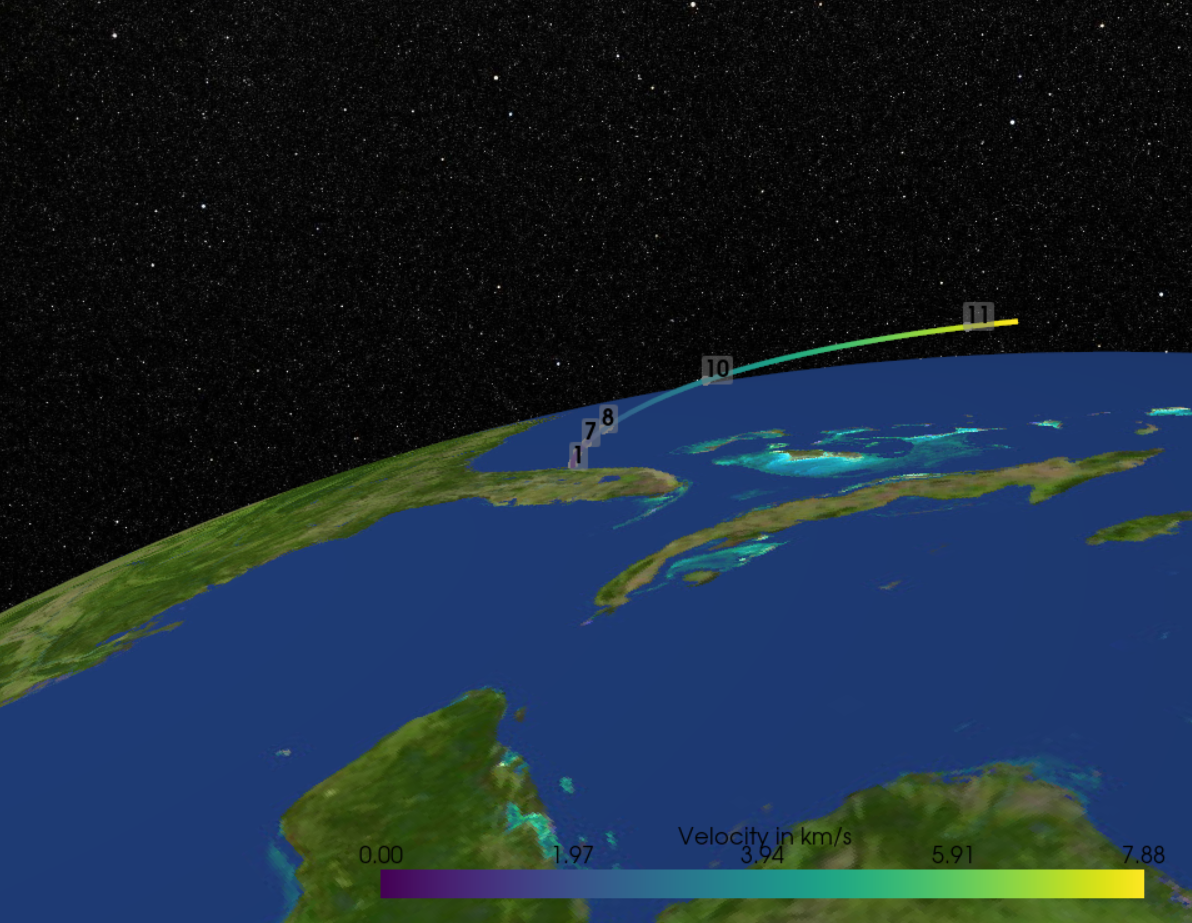
\includegraphics[width=\textwidth]{images/example-plot.png}
  \caption{The example trajectory shown with the plotting tool. The color
    indicates the velocity of the vehicle while the labels indicate the start of a
    new phase.}
  \label{example-plot}
\end{figure}

\paragraph{Example}

The original documentation also included an example trajectory for the ascent
of a space shuttle type vehicle. This example is used to validate this
project.

The example is included in \lstinline{sim\src\utils\input.json}. It can be used as a starting point for custom configurations.

To execute the example, run:
\begin{lstlisting}[language=sh]
 $ target\release\post.exe --config sim\src\utils\input.json | python sim\src\utils\plot\plot.py
\end{lstlisting}

\subsection{Configuration File}\label{configuration-file}

The \gls{json} configuration file consists of an array of configurations, one for
each phase. Each phase is inheriting the configuration of the previous phase.
Then the specified parameters are overwritten.

As the first phase does not have a previous phase, there is a default phase to
inherit from:

\begin{lstlisting}[language=json,mathescape]
 [
   {
     "planet_model": "spherical",
     "atmosphere": {
       "enabled": false,
       "wind": [ 0, 0, 0 ] // in m/s
     },
     "init": {
       "latitude": 0, // in $\text{°}$
       "longitude": 0, // in $\text{°}$
       "azimuth": 0, // in $\text{°}$
       "altitude": 0 // in m
     },
     "vehicle": {
       "structure_mass": 0, // in kg
       "propellant_mass": 0, // in kg
       "reference_area": 0, // in m^2
       "drag_coeff": {"x": ["time", []], "data": []},
       "lift_coeff":  {"x": ["time", []], "data": []},
       "side_force_coeff":  {"x": ["time", []], "data": []},
       "engines": [
           {
             "incidence": [ 0, 0 ], // in rad
             "thrust_vac": 0, // in N
             "isp_vac": 0, // in s
             "exit_area": 0 // in m^2
           }
         ]
       },
       "max_acceleration": -1, // in m/s^2, -1 for disabling
       "steering": {
       "roll": [ "time", [ 0, 0, 0 ] ], // in $\text{°}$
       "yaw": [ "time", [ 0, 0, 0 ] ], // in $\text{°}$
       "pitch": [ "time", [ 0, 0, 0 ] ]  // in $\text{°}$
     },
     "stepsize": 0, // in s
     "end_criterion": [ "time", 0 ]
   },
   { ... },
   ...
 ]
\end{lstlisting}

Overwriting the propellant mass will also reset the consumed propellant.

Setting a parameter to \json{null} is the same as not specifying it, so it will not be overwritten.

\paragraph{Planet model}

The planet model has 4 valid parameters:
\json{"spherical"}, \json{"fisher_1960"}, \json{"smithsonian"}, or a custom model. A custom planet model must be
specified with:

\begin{lstlisting}[language=json]
 {
   "custom": {
     "equatorial_radius": 6.3781658568e6, // in m
     "polar_radius": 6.356783832e6, // in m
     // [mu, J_2, J_3, J_4]
     "gravitational_parameters": [
         1.3077457350581376e15, // in m^3/s^2
         1.082639e-3,
         -2.565e-6,
         -1.608e-6,
     ],
     "rotation_rate": 7.29211e-5, // in rad/s
   }
 }
\end{lstlisting}

\begin{quote} Here, the Smithsonian model implementation is shown.
\end{quote}

\paragraph{Steering}

The steering configuration are the coefficients \(c_i\) for a cubic
polynomial of the form \[
  \alpha = c_0 + c_1y + c_0y^2 + c_1y^3.
\] The first coefficient \(c_0\) is initialized as zero for the first
phase. For later phases, it is initialized as the last Euler angle of
the previous phase. This is done to avoid jumps in the orientation.

The variable \(y\) is any simulation variable. Following variables are
defined:

\paragraph{Simulation Variables}

\begin{longtable}{l l}\json{"time"}                      & Simulation time                                                                  \\
                 \json{"time_since_event"}               & Time since the last event                                                        \\
                 \json{"position1"}                      & Inertial position                                                                \\
                 \json{"position2"}                      &                                                                                  \\
                 \json{"position3"}                      &                                                                                  \\
                 \json{"position_norm"}                  & Distance from earth center                                                       \\
                 \json{"position_planet1"}               & Earth-relative position                                                          \\
                 \json{"position_planet2"}               &                                                                                  \\
                 \json{"position_planet3"}               &                                                                                  \\
                 \json{"altitude"}                       & Height above surface                                                             \\
                 \json{"altitude_geopotential"}          & Used for the atmospheric model\footnote{Calculated with \(\frac{R_Ah}{R_A+h}\).} \\
                 \json{"velocity1"}                      & Inertial velocity                                                                \\
                 \json{"velocity2"}                      &                                                                                  \\
                 \json{"velocity3"}                      &                                                                                  \\
                 \json{"velocity_norm"}                  & Total inertial velocity                                                          \\
                 \json{"velocity_planet1"}               & Earth-relative velocity                                                          \\
                 \json{"velocity_planet2"}               &                                                                                  \\
                 \json{"velocity_planet3"}               &                                                                                  \\
                 \json{"velocity_planet_norm"}           & Total earth-relative velocity                                                    \\
                 \json{"velocity_atmosphere1"}           & Atmosphere-relative velocity                                                     \\
                 \json{"velocity_atmosphere2"}           &                                                                                  \\
                 \json{"velocity_atmosphere3"}           &                                                                                  \\
                 \json{"velocity_atmosphere_norm"}       & Total atmosphere-relative velocity                                               \\
                 \json{"acceleration1"}                  & Inertial acceleration                                                            \\
                 \json{"acceleration2"}                  &                                                                                  \\
                 \json{"acceleration3"}                  &                                                                                  \\
                 \json{"acceleration_norm"}              & Total inertial acceleration                                                      \\
                 \json{"thrust_force_body1"}             & Thrust force in body frame                                                       \\
                 \json{"thrust_force_body2"}             &                                                                                  \\
                 \json{"thrust_force_body3"}             &                                                                                  \\
                 \json{"thrust_force_body_norm"}         & Total thrust force in body frame                                                 \\
                 \json{"aero_force_body1"}               & Aerodynamic force in body frame                                                  \\
                 \json{"aero_force_body2"}               &                                                                                  \\
                 \json{"aero_force_body3"}               &                                                                                  \\
                 \json{"aero_force_body_norm"}           & Total aerodynamic force in body frame                                            \\
                 \json{"vehicle_acceleration_body1"}     & Vehicle sensed acceleration                                                      \\
                 \json{"vehicle_acceleration_body2"}     & \(\hookrightarrow\) Acceleration due to thrust and aero forces                   \\
                 \json{"vehicle_acceleration_body3"}     &                                                                                  \\
                 \json{"vehicle_acceleration_body_norm"} & Total vehicle senses acceleration                                                \\
                 \json{"gravity_acceleration1"}          & Acceleration due to gravity                                                      \\
                 \json{"gravity_acceleration2"}          &                                                                                  \\
                 \json{"gravity_acceleration3"}          &                                                                                  \\
                 \json{"gravity_acceleration_norm"}      & Total acceleration due to gravity                                                \\
                 \json{"mass"}                           & Total vehicle mass                                                               \\
                 \json{"propellant_mass"}                & Propellant mass                                                                  \\
                 \json{"massflow"}                       & Propellant massflow                                                              \\
                 \json{"temperature"}                    & Atmosphere temperature                                                           \\
                 \json{"pressure"}                       & Atmosphere pressure                                                              \\
                 \json{"density"}                        & Atmosphere density                                                               \\
                 \json{"mach_number"}                    & Vehicle mach number                                                              \\
                 \json{"dynamic_pressure"}               & Dynamic pressure                                                                 \\
                 \json{"alpha"}                          & Angle of attack                                                                  \\
                 \json{"euler_angles_roll"}              & Roll angle with respect to launch frame                                          \\
                 \json{"euler_angles_yaw"}               & Yaw angle with respect to launch frame                                           \\
                 \json{"euler_angles_pitch"}             & Pitch angle with respect to launch frame                                         \\
                 \json{"throttle"}                       & Computed auto-throttle                                                           \\
\end{longtable}

\paragraph{Aerodynamic coefficients}

Aerodynamic coefficients are input as tables. There are 1D, 2D and 3D tables,
which are structured as follows:

\textbf{1D:}

\begin{lstlisting}[language=json]
 {
   "x": ["<state var>", [ ... ]],
   "data": [ ... ]
 }
\end{lstlisting}

\textbf{2D:}

\begin{lstlisting}[language=json]
 {
   "x": ["<state var>", [ ... ]],
   "y": ["<state var>", [ ... ]],
   "data": [ [ ... ] ]
 }
\end{lstlisting}

\textbf{3D:}

\begin{lstlisting}[language=json]
 {
   "x": ["<state var>", [ ... ]],
   "y": ["<state var>", [ ... ]],
   "z": ["<state var>", [ ... ]],
   "data": [ [ [...] ] ]
 }
\end{lstlisting}

Note that the \json{"data"} parameter changes: A 1D table uses an array, a 2D table an array
of arrays and a 3D table an array of arrays of arrays.

For the \json{"x"}, \json{"y"} and \json{"z"} variables, any simulation variable (defined above) can be specified.
This will then be used to interpolate between the data points.

\section{Discussion}\label{discussion}

In this chapter, I will discuss the differences of this project to the
original. Also, I will outline my thoughts about the programming language of
my choice for this project, Rust.

\subsection{Differences to the original}\label{differences-to-the-original}

While I tried to closely follow the original, some things differ. Mostly, not
all features were implemented. This is further detailed in this chapter.

\subsubsection{Missing Features}\label{missing-features}

The original program includes a lot of features and multiple options for many
of them. As time is limited, this project only implemented the most important
ones (the ones needed to simulate the example space shuttle trajectory). Some
of these missing features might be implemented in the future, but most of them
are deemed unnecessary for now.

\paragraph{Initialization}

While this project only includes initialization using geodetic latitude,
longitude and altitude, the original program also included initialization with
inertial position and velocity, with orbit parameters and a few others. The
most important of which are planned to be implemented in the future.

\paragraph{Steering}

In the original program, the vehicle could be steered using angular rates,
aerodynamic angles, relative Euler angles and inertial aerodynamic angles.
They could be calculated with (cubic) polynomials, tables, or even by
implementing a custom feedback controller. While most of these are not
considered to be implemented, a 6 \glspl{dof} version would be interesting which would come with big changes to
the steering model.

\paragraph{Additional calculations}

The original program would calculate a bunch of additional variables for each
time step, which partly could be used as inputs for steering or tables. These
included a heating model, orbit parameters, range calculations, ground station
visibility, sun and shadow calculations and others. These are not essential,
but the most important of them are planned to be implemented sometime in the
future.

\paragraph{Atmosphere models}

In the original program, one could also use a custom atmosphere model
specified with tables and the 1963 Patrick AFB model. These will most likely
never be implemented, but rather a more modern model.

\paragraph{Jet engines}

The original program could also simulate jet engines. As I am mostly
interested in space travel, they will most likely not be implemented in the
future.

\paragraph{Events}

The original program included some more options to specify events, like
optional or repeating events. As these are only needed for more complex
missions, they are in the backlog for now.

\paragraph{Integrators}

The original program included more options for integrators like the Krogh
Integrator, the Laplace method or Encke's method. These will be implemented
only if necessary.

\subsubsection{Auto-throttling}\label{auto-throttling}

The original documentation is very detailed regarding the simulation and can
be followed without big difficulty. There is, however, one part which I did
not find any explanation about, which is the auto-throttling.

The user can specify a maximum sensed acceleration, which should not be
exceeded. To ensure this, the thrust is throttled automatically. The algorithm
to calculate the throttle had to be designed by myself, which works as
follows.

\paragraph{Problem statement}

\gls{A_TB} and \gls{A_AB}, together with the resulting \gls{A_SB} form a triangle in 3D space, as seen in \cref{auto-throttle}. \gls{A_AB} can be calculated with \gls{v_I}, while the the magnitude of \gls{A_SB} should not exceed a maximum value. Also, the direction of \gls{A_TB} is known from the thrust incidence angles \gls{i_y} and \gls{i_p}.

\begin{figure}[!ht]
  \centering
  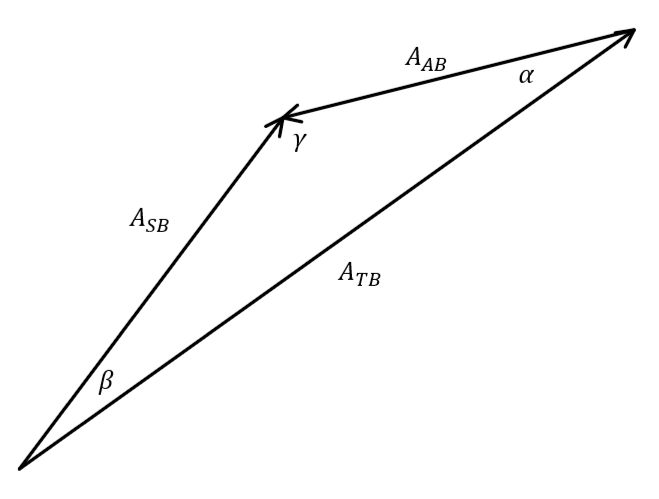
\includegraphics[width=0.5\textwidth]{images/auto-throttle.png}
  \caption{The auto-throttling problem.}
  \label{auto-throttle}
\end{figure}

\paragraph{Solution}

Using the direction of \gls{A_TB} and \gls{A_AB}, the angle between the two vectors \(\alpha\) can be calculated. Now the magnitude of \gls{A_AB} and \gls{A_SB} is given together with an angle. This means we can calculate all
values in the triangle with the side-side-angle method.

Using the law of sines with
\(\alpha\), \gls{A_AB} and \gls{A_SB}, a second angle \(\beta\) can be
calculated, which is opposite of \gls{A_AB}. The third angle \(\gamma\)
trivially follows, as all angles add up to 180° or \(\pi\).

Finally, the law of sines can be used again to calculate \gls{A_TB}, using
\gls{A_AB}, \(\beta\) and \(\gamma\).

Lastly, one has to catch all the edge cases, and make sure the resulting
\gls{A_TB} is not negative or bigger than the maximum possible \gls{A_TB} using full thrust.

\subsection{The programming language used:
  Rust}\label{the-programming-language-used-rust}

Rust was chosen for this project for a few simple reasons.

First, Rust is fast\cite{Benchmarks, BenchmarksGame}. Its speed is easily comparable with C and
C++. As this project is about an optimization of a complex simulation, speed
is very likely of importance.

Also, Rust is safe. Its unique borrow checker and strong type system allows
you to write reliable, safe and less buggy code more easily. This takes away
the nightmare of having to debug memory related bugs, like with C or C++.
Basically, it is much harder to shoot yourself in the foot.

But most importantly, I wanted to try out and learn Rust. Rust is the
consecutive most loved programming language for 8 years in a row, according to \cite{StackOverflow2023}, which piqued my interest. Also, as I mostly work with
Python, I wanted to add a fast, low-level programming language to my arsenal.

\subsubsection{The Good}\label{the-good}

This chapter is inherently opinion based. This chapter is only about how I
experienced working with and learning the language and are exaggerated a bit
to underline my points. Some issues can very much boil down to me not having
enough experience with the language, or with low-level languages in general.

First things first, I think Rust is doing a lot of things right. There are a
bunch of things great about the language. Like, as already mentioned, the
safety does free you from some annoying bugs. But sometimes overlooked, I
believe the environment of a programming language is sometimes more important
than the language itself. And here, Rust really shines.

There exists a central tool for downloading, installing and updating the Rust
language, compiler, package manager and tools, called ``rustup''.

The best part is the package manager, called ``Cargo''. It is used to run all
the tools that already come with Rust. It can be used to create a new project,
build and run your code, test or benchmark it, download packages and add it to
your dependencies. It is used for linting and formatting, to create automatic
documentation and even publish it to Rust's package index.

Languages like Python also have all of these features, but in Rust, most of
them are already coming with your installation, ready to use. Or more
importantly, there is one ``official'' tool for all of these tasks. I mostly
do not care how to format my code, I only want it to be easy and uniformly
across all projects. The exact formatting rules don't matter, as long as they
are officially declared.

There is also one way to declare dependencies, give additional information
about the project and publish your code and documentation. Speaking of
documentation, automatic documentation from code comments is already built-in,
even with examples which are automatically tested! And the documentation can
then be published on an official site which is linked with the package index.

\subsubsection{The Bad}\label{the-bad}

In my experience with this project, Rust can be very clunky and writing it is
slow. While this certainly gets better with more experience, I believe it will
always make your life hard in certain scenarios. Also, I believe the learning
experience should be considered when evaluating a programming language, which
can feel like an uphill battle in Rust. While there were many instances where
the language was standing in the way of how I wanted to solve a problem, a few
examples are detailed here.

Rust's speed can be quickly compromised (and probably is in many parts of this
project) by an exhausted developer who does not want to fight the borrow
checker anymore and simple clones a rather big structure.

Also, dealing with slightly complex structures is a nightmare. One example for
this are the tables used for the aerodynamic coefficients. At first, these
were implemented recursively. A 3D table consisted of a number of 2D tables,
and so on. Working out how build the structure was already complex, but
manageable. The problems began, once these tables needed to be cloneable: The
tables were owned by the vehicle struct. Because the type must be known, the
tables were a generic type, restricted by a shared trait. Because it was
infeasible to copy the type restriction of the generic (meaning the
specification of the trait) across the entire project, the trait was
``dynamically dispatched''. This then in turn restricts the trait to be
`object safe', which is what being cloneable is not\footnote{This can be circumvented with the
  \lstinline{dyn_clone} crate. The implementation fell apart, though, when the
  tables needed to be deserializable. Again, deserialization is not object safe,
  but can be again be circumvented with
  \lstinline{erased_serde}. But I spend about a week to figure out how to
  deserialize a recursive structure, without knowing which type it is
  beforehand. So I figured it is not worth it and abandoned the (in my eyes more
  elegant) implementation of the tables.}.

\subsubsection{The Verdict}\label{the-verdict}

I believe Rust is a great language, if applied to the right problems.

Before considering Rust, it needs to be clear that its speed is really needed.
Also, the problem should not require too many complex, nested or recursive
data structures. I think Rust really shines for low-level high-intensity tasks
and complemented by high-level languages which handle the encompassing logic.

\section{Development}\label{development}

The project is still in development. Currently, the simulation part of the
program is functional, but the optimization part is still missing.

Other than that, there still exists some known issues and some changes are
planned. While these are tracked in the
\href{https://github.com/TiborVoelcker/post/issues}{issues}, the most important
ones are outlined below.

To read more about the code of the project, visit the
\href{https://tiborvoelcker.github.io/post/docs/post/index.html}{code documentation}.

\paragraph{Existing Issues}\label{existing-issues}

\begin{itemize}
  \item Program panics when reaching max. acceleration
  \item Unspecified behavior for negative altitudes
  \item Unspecified behavior or crashing for invalid configuration (e.g.~zero
        mass)
  \item Unlimited simulation duration if end condition is never reached (or was
        reached before event started)
  \item Thrust is generated even when propellant was consumed
  \item Bad performance due to writing to stdout, unnecessary cloning or passing
        by value
\end{itemize}

\paragraph{Planned Changes and Features}\label{planned-changes-and-features}

\begin{itemize}
  \item Output timesteps as a table
  \item Let output be configurable
  \item Improve logging using the \lstinline{log} crate
  \item Improve code documentation with comments and examples
  \item Include plotting script into the \gls{cli}
  \item Add figures for e.g.~orientation in the plotting script
  \item Add safety against unit (rad vs °) or frame differences (inertial vs
        relative)
\end{itemize}
